% Q8 Answer
\clearpage
\section*{Question 8}
\addcontentsline{toc}{section}{Question 8}

Using variable-step solvers, set $h_{max} = 1 \times 10^{-2}$ and both error tolerances $\varepsilon_{abs} = \varepsilon_{rel} = 10^{-3}$. Experiment with all the available variable-step solvers. In a table, print the maximum time-step size $h_{max}$ chosen by each solver and the total number of steps taken. Comment on how these solutions compare with the reference solution found in part 7. Which solver in your opinion is more efficient and does the best job for this system? Compare the step-size and the overall number of steps observed in parts 6, 7, and this part.

\subsection*{Figures and Analysis}
The following figures illustrate the transient response of the inductor current $i_L(t)$ and capacitor voltage $V_C(t)$ for both nonstiff and stiff solvers. \Cref{fig:transient_response_all} includes all solvers, highlighting the performance of solvers that fail to dampen oscillations effectively. \Cref{fig:transient_response_good} excludes these solvers, focusing only on the solvers that converge to the expected damped sinusoidal response:

\begin{figure}[h!]
    \centering
    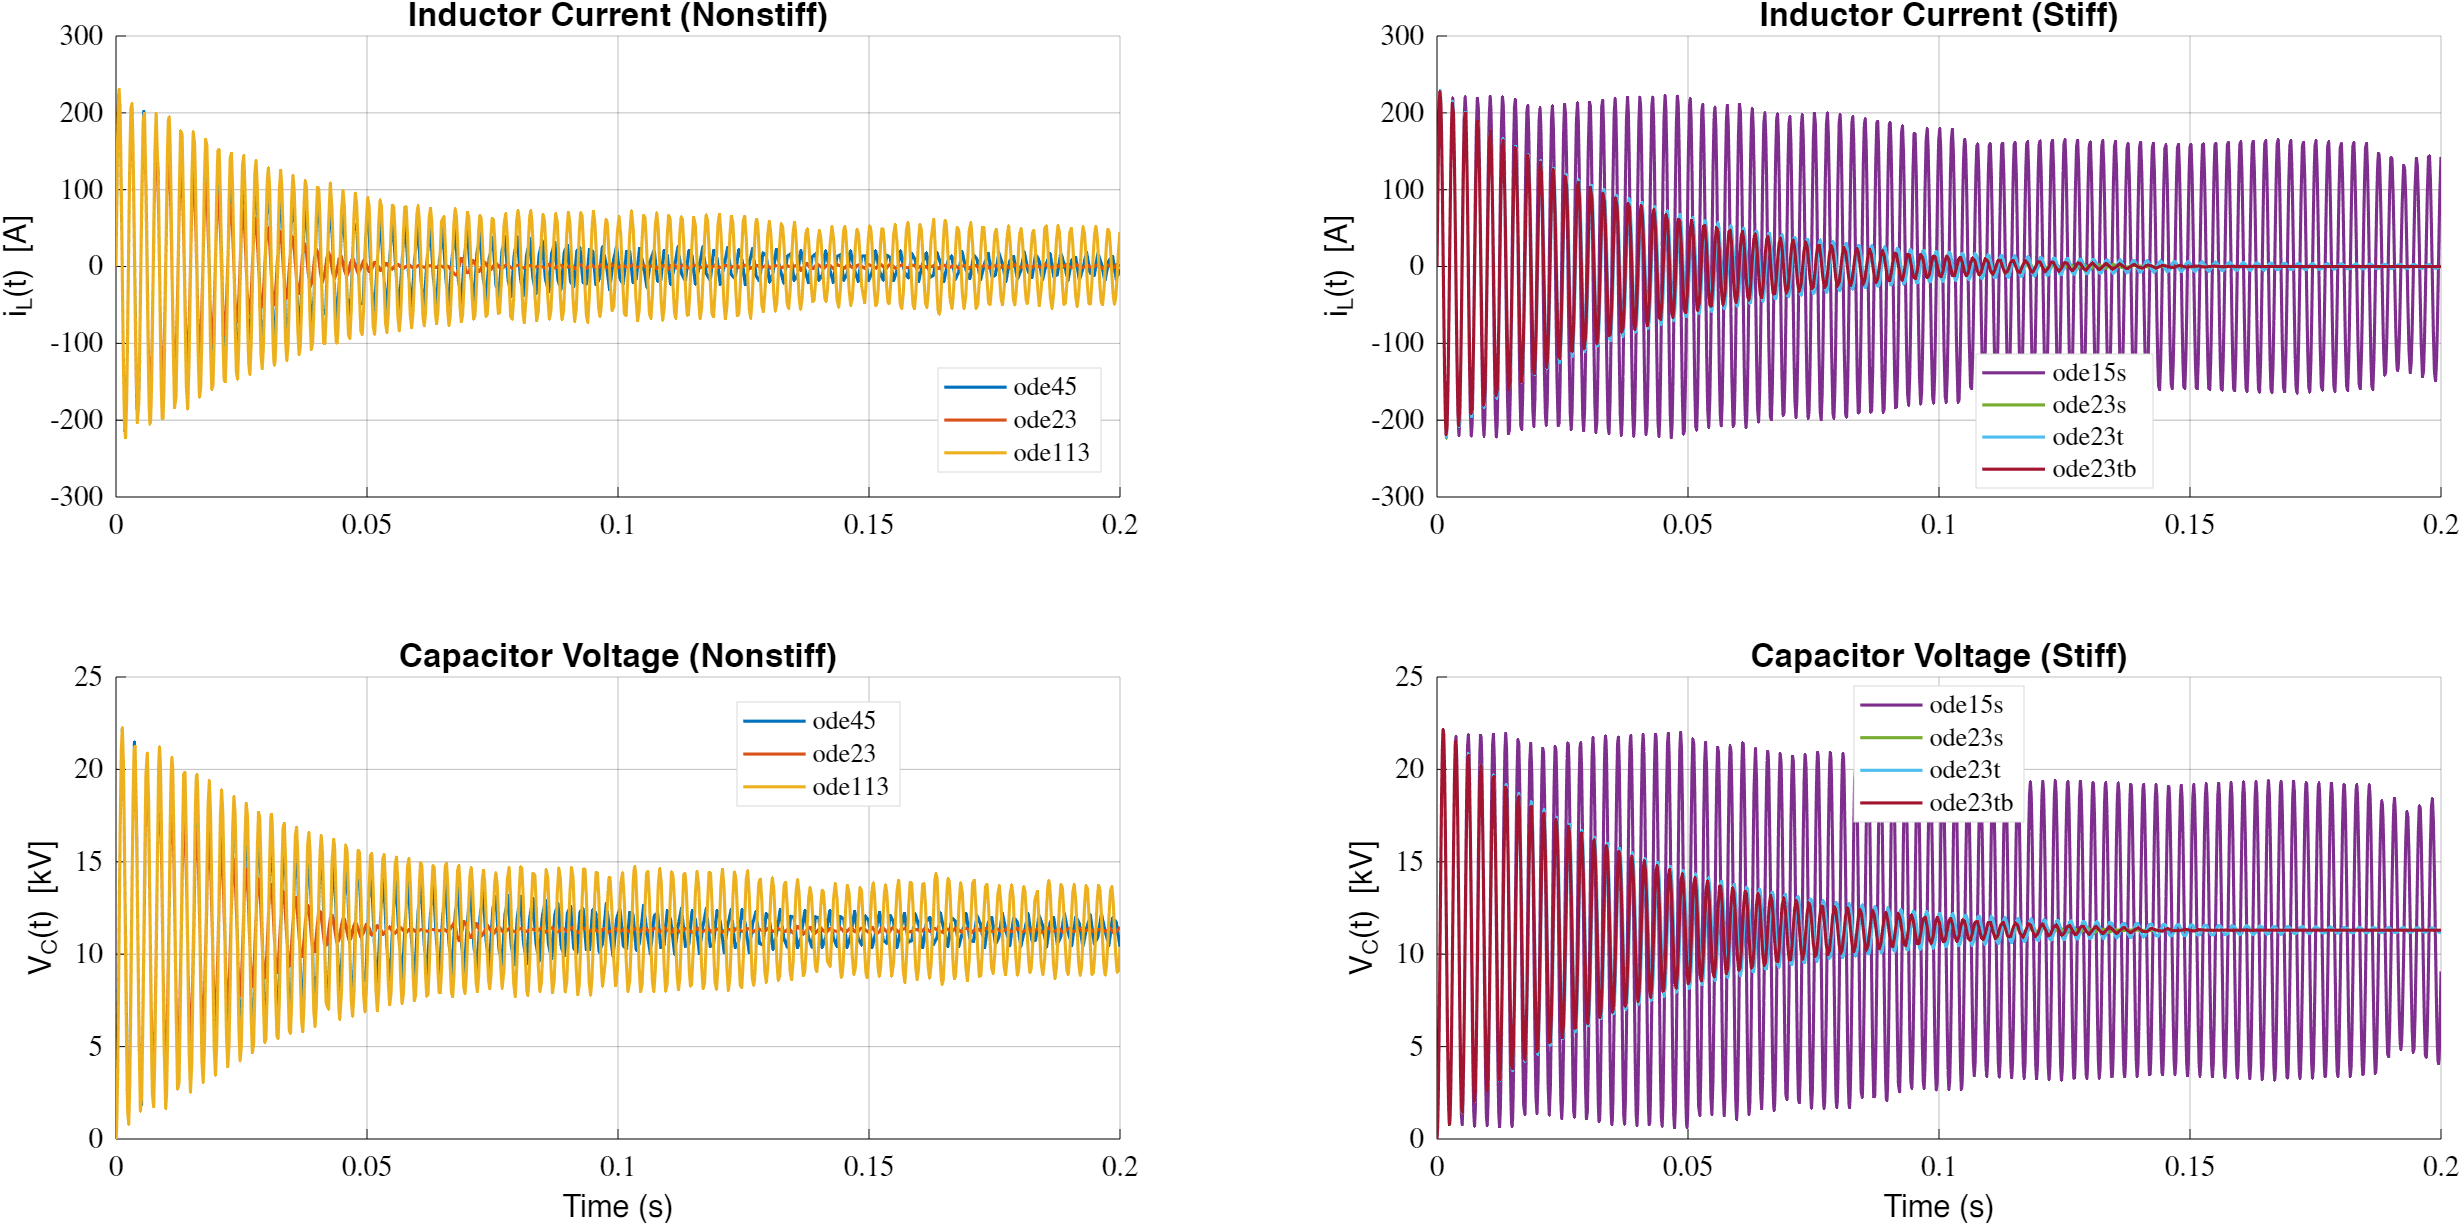
\includegraphics[width=0.8\textwidth]{figures/hw01_q08_plots-of-iL-and-Vc-for-different-variable-step-ode-solvers.png}
    \caption{Transient Response of Inductor Current and Capacitor Voltage (Including Non-Dampening Solvers)}
    \label{fig:transient_response_all}
\end{figure}

\begin{figure}[h!]
    \centering
    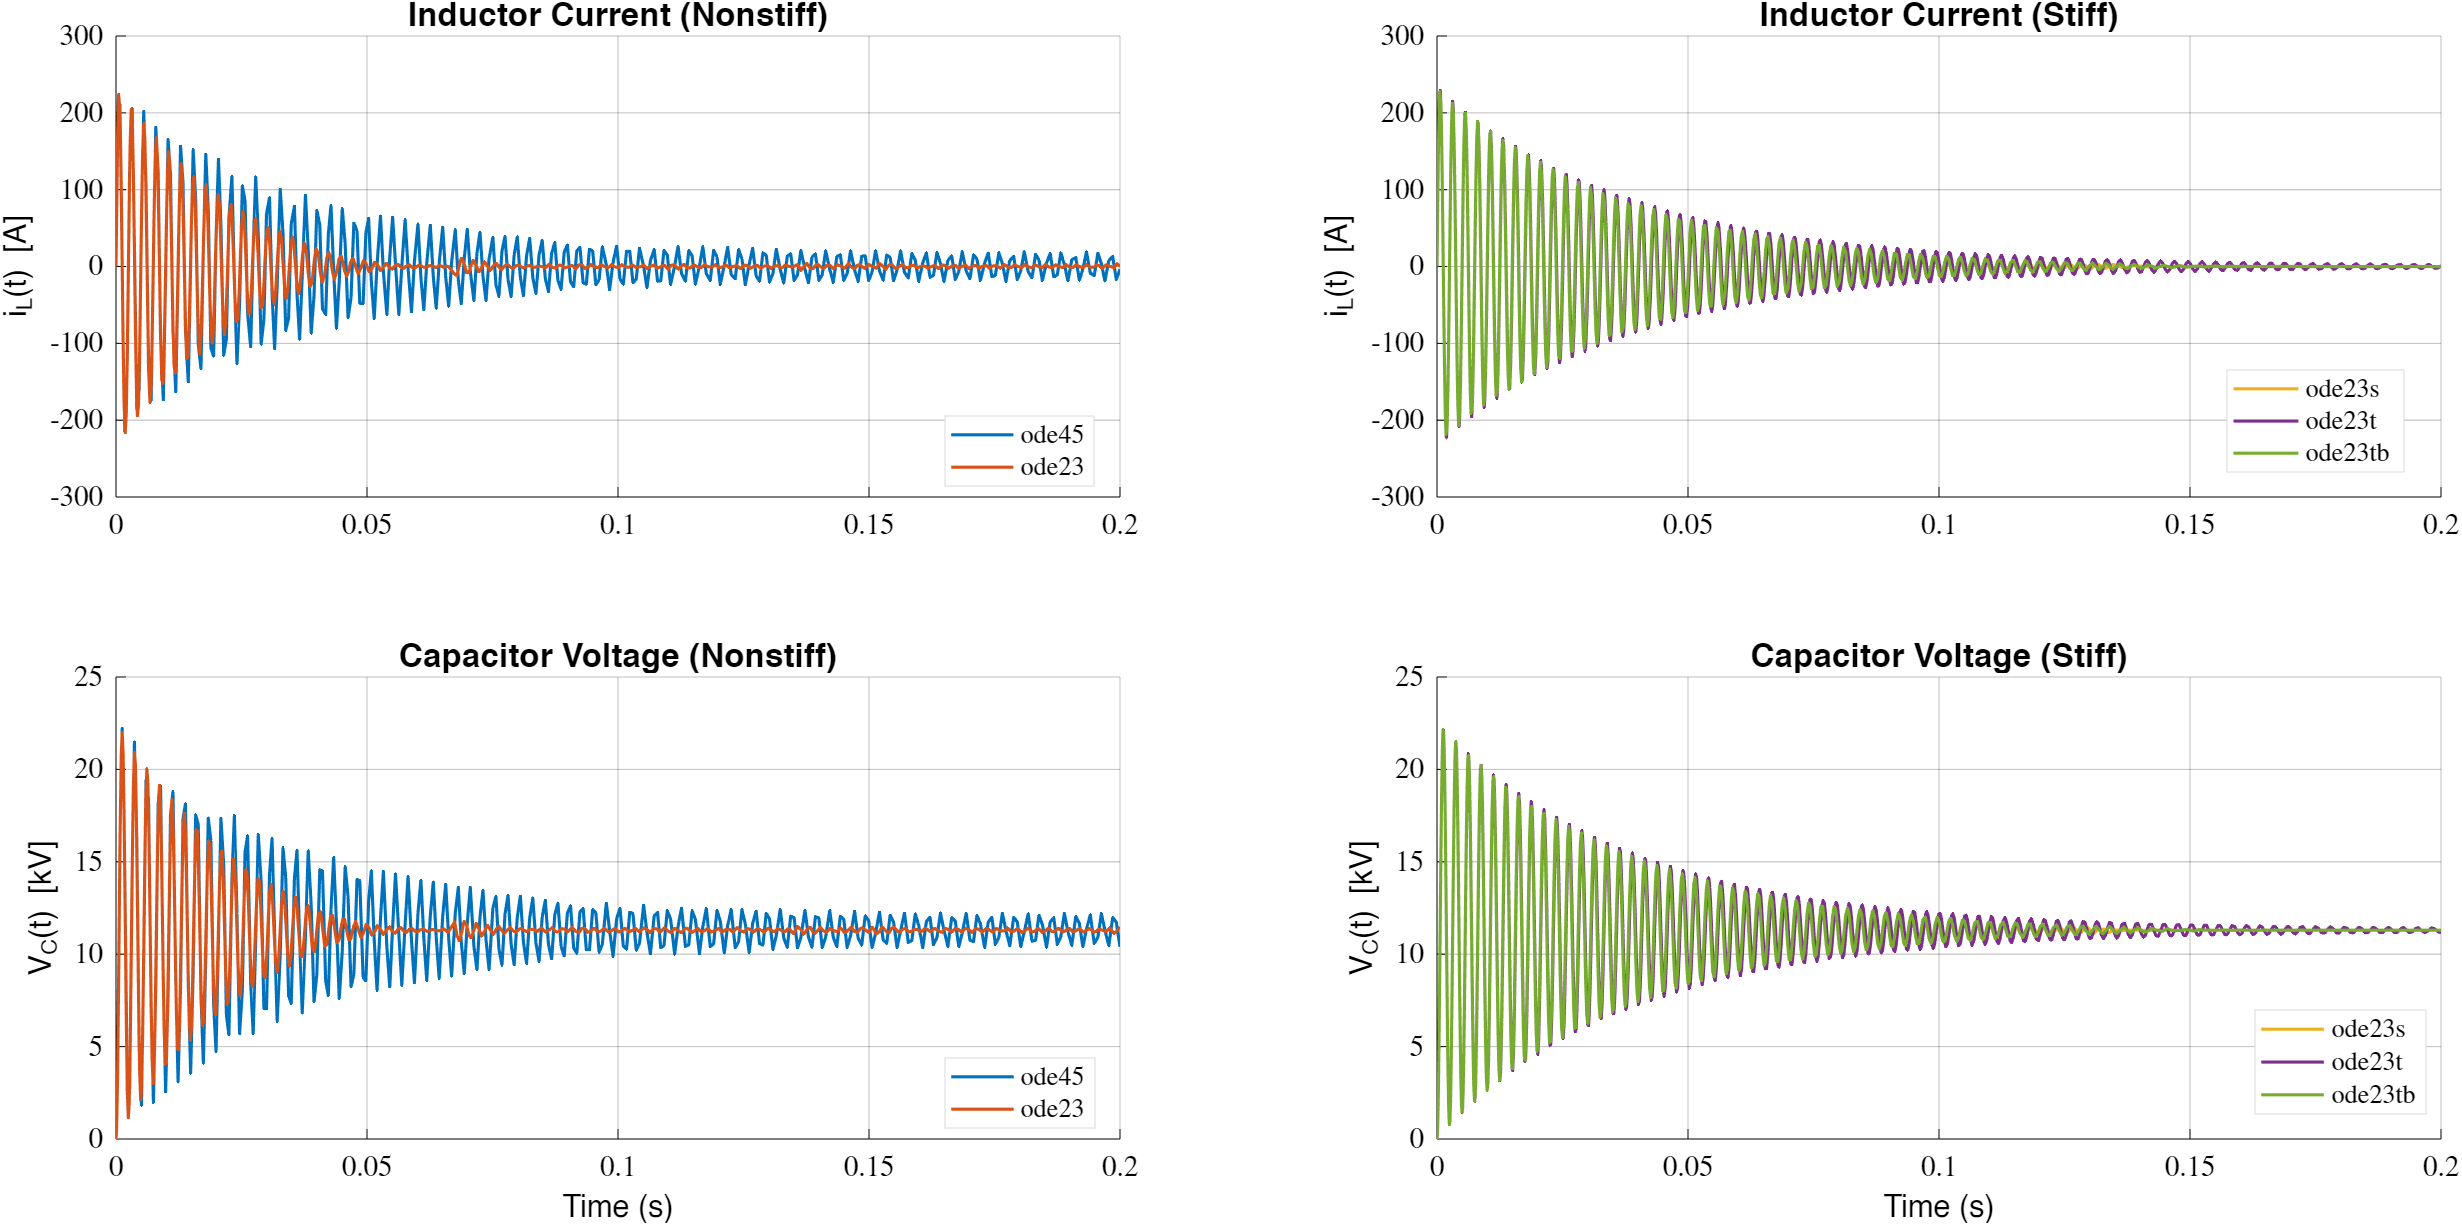
\includegraphics[width=0.8\textwidth]{figures/hw01_q08_plots-of-iL-and-Vc-for-different-variable-step-ode-solvers-only-good_Thorizon_0_2s.png}
    \caption{Transient Response of Inductor Current and Capacitor Voltage (Excluding Non-Dampening Solvers)}
    \label{fig:transient_response_good}
\end{figure}

% Added image before the table to establish authenticity
\begin{figure}[h!]
    \centering
    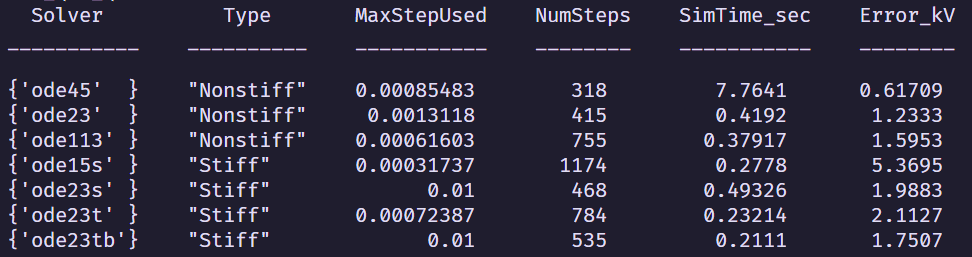
\includegraphics[width=0.8\textwidth]{figures/hw01_q08_table-comparing-metrics-for-different-variable-step-ode-solvers.png}
    \caption{Simulation Results for Variable-Step ODE Solvers}
    \label{fig:simulation_results_table}
\end{figure}

\subsection*{Table of Results}
The table below, supported by \cref{fig:simulation_results_table}, summarizes the performance of each solver, including the maximum step size used, the number of steps taken, the simulation time, and the RMSE error:

\begin{table}[h!]
    \centering
    \begin{tabular}{|l|l|c|c|c|c|}
        \hline
        \textbf{Solver} & \textbf{Type} & \textbf{$h_{Max}$} & \textbf{Num Steps} & \textbf{Time [s]} & \textbf{Error [kV]} \\
        \hline
        ode45 & Nonstiff & 0.0008548 & 318 & 7.7641 & 0.6171 \\
        ode23 & Nonstiff & 0.0013118 & 415 & 0.4192 & 1.2333 \\
        ode113 & Nonstiff & 0.0006160 & 755 & 0.3792 & 1.5953 \\
        ode15s & Stiff & 0.0003174 & 1174 & 0.2778 & 5.3695 \\
        ode23s & Stiff & 0.01 & 468 & 0.4933 & 1.9883 \\
        ode23t & Stiff & 0.0007239 & 784 & 0.2321 & 2.1127 \\
        ode23tb & Stiff & 0.01 & 535 & 0.2111 & 1.7507 \\
        \hline
    \end{tabular}
    \caption{Summary of Solver Performance}
    \label{tab:solver_performance}
\end{table}

\subsection*{Discussion}
While nonstiff solvers (ode45, ode23) generally showed lesser error and had better timings, their transient response 'shape' was less consistent with a damped sinusoid as expected from the analytical solution. Stiff solvers (ode15s, ode23s) produced responses that visually aligned better with the expected damped sinusoidal shape, but they exhibited higher numerical error and longer computation times. Still, I personally found any stiff solver variation of ode23 (ode23s, ode23t, ode23tb) to be the best compromise between accuracy, speed, and expected response shape.

Among the stiff solvers, the variations of ode23 (ode23s, ode23t, ode23tb) stood out as a balanced choice. These solvers demonstrated a reasonable trade-off between computational efficiency and the ability to replicate the expected transient response shape.

\subsection*{Remarks on Error Computation}
The error metric used in this analysis is the root mean square error (RMSE), computed by evaluating the analytical solution at the same time steps as those of the numerical solver. The analytical solution, derived in Q2, is given by:
\begin{align*}
    V_{c}(t) [kV] = 11.3 \left[1 - 1.00005 \, e^{-26.34\, t} \, \sin(2533.3\, t + 1.5604)\right]
\end{align*}
This approach ensures a fair comparison, as the error is calculated point-by-point at identical time instances.

\subsection*{Performance Observations}
One notable observation is the computational inefficiency of ode45, which, despite its small maximum step size, takes significantly longer to compute the solution compared to other solvers. This inefficiency is likely due to its explicit Runge-Kutta method, which requires more function evaluations per step.

Among the stiff solvers, the ode23 line (ode23s, ode23t, ode23tb) consistently demonstrated better performance in terms of balancing accuracy and computational time. While the timings for these solvers vary slightly between runs, they generally remain within a similar range, making them a reliable choice for stiff systems.

In conclusion, the stiff solvers, particularly the ode23 variants, are recommended for this problem due to their ability to handle rapid dynamics efficiently while maintaining accuracy.
